\chapter{Introduction}
This chapter introduces the assignment and some foundational concepts of quantum sensing.

\section{Background}
Nitrogen-vacancy (NV) centers \cite{enwiki:1301369588} are imperfections in the atomic structure of diamonds. The two types of NV centers are NV0 and NV-, as seen in Figure \ref{fig:nvcenter}, but the NV- structure is much more commonly used in quantum applications. These imperfections have the useful property of spin-dependent luminescence. This means that the spin of the NV center affects the frequency of the light emitted by the structure\footnote{The NV center only emits light after absorbing photons, a phenomenon called photoluminescence \cite{enwiki:1309081879}}. Using this quality of the NV structure, different environmental metrics (e.g magnetic fields) can be measured. 

The Applied Nanotechnology research group is working on a NV-center-based sensor setup. There exist several quantum protocols, but the one this setup needs to support is called Continuous-Wave Optically Detected Magnetic Resonance (CW-ODMR). At its core, ODMR is a set of protocols, which can detect magnetic fields based on the fluctuations in the fluorescence of NV centers \cite{enwiki:1301371272}. CW-ODMR in particular involves exposing the NV center to a MicroWave (MW) sweep while illuminating it with a constant light source. This is in contrast with pulsed ODMR techniques, which use different TTL (transistor-transistor logic) pulse schemes \cite{sewani2020coherent} to modulate the MW signal and the light source.

Processing data from the setup requires working with weak signals that are hard to distinguish from the environmental noise. While this is a significant problem, it is also a very common one. Because of this, there is already widely-used system used to isolate signals in such cases: the lock-in amplifier.

\begin{figure}[ht]
	\centering
	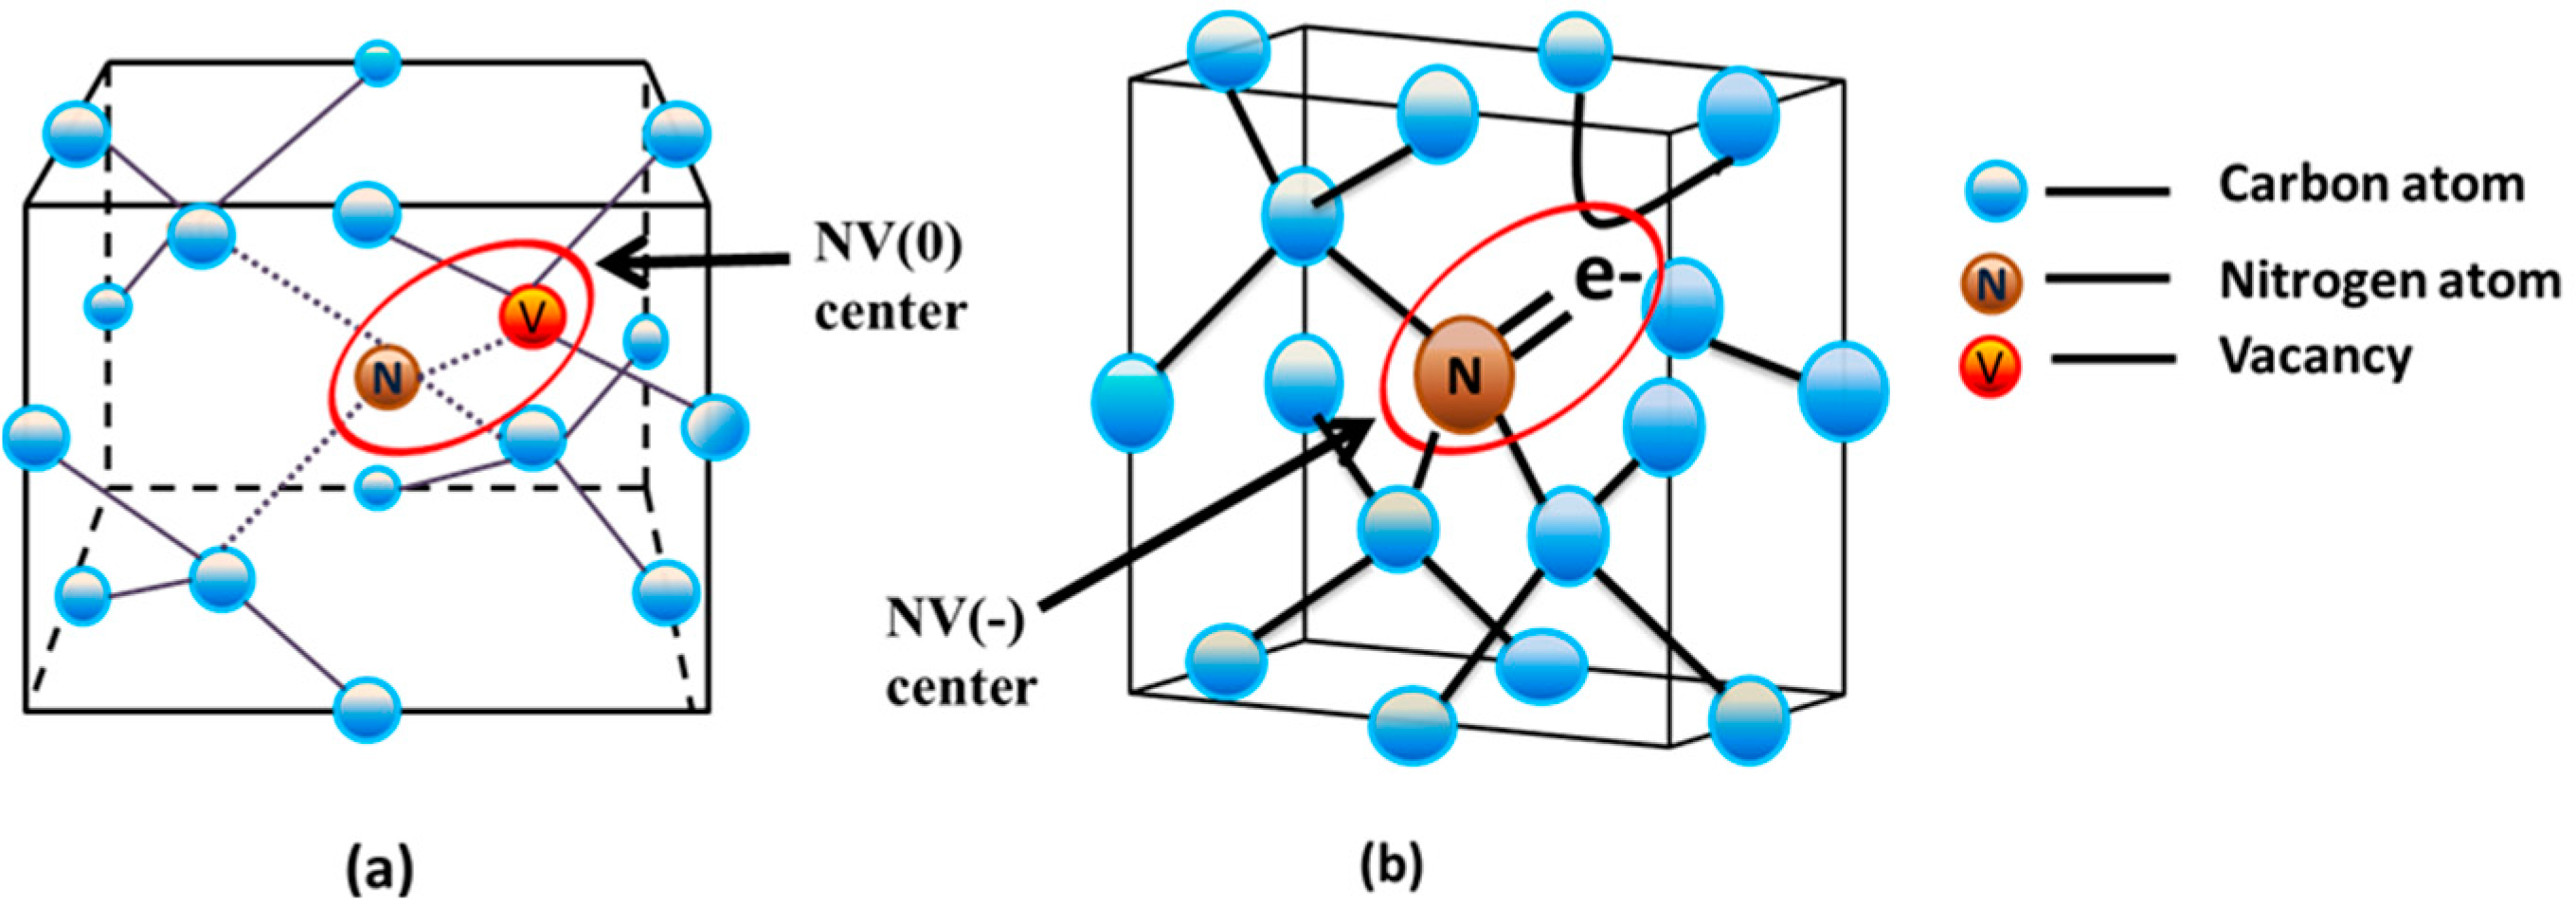
\includegraphics[width=0.7\linewidth]{img/nv_center}
	\caption{NV0 (a) and NV- (b) structures in diamonds (image credit to Haque et al \cite{haque2017overview})}
	\label{fig:nvcenter}
\end{figure}


\section{Purpose of the assignment}\label{purpose}
Implementing a lock-in amplifier is the main purpose of the assignment. To create a complete solution, there are several different functionalities and systems that need to be developed. 

Before doing anything else, the raw sensor data needs to be extracted and then fed to a lock-in amplifier. This should be done in a standardized manner, in order to facilitate testing with different devices. After establishing connection, a control interface needs to be implemented. It needs to be programmed so that it can control all necessary features of the lock-in amplifier. Following the development of the program, a custom photodetection circuit needs to be designed. The circuit should accommodate the sensors and lock-in amplifier. Lastly, an OLIA\footnote{Open Lock-In Amplifier (OLIA) is an open-source microcontroller-based lock-in amplifier. It uses common components, which makes it easy to build \cite{harvie2023olia}} circuit needs to be tested and compared to conventional lock-in systems. 


\section{Assignment specifications}\label{specifications}
As already explained, the assignment is quite broad and involves both hardware and software, causing the need for a number of different tools. 

Most of the hardware tools are already available at the Applied Nanotechnology lab. The lock-in amplifiers which will be used for the tests are the most important pieces of hardware. Zurich Instruments HF2LI is the benchmark lock-in amplifier. The target amplification is at least 10dB. There are also several different photodetectors available and the one which fits the project best will be picked at a later date. Chapter \ref{chap:background} already discussed the basics of the CW-ODMR protocol. In order to get an operational CW-ODMR setup, an MW generator and a laser will be used. MW sweeping needs to be done in the range of 2,8 - 2,9 GHz and the lab already has a custom-built MW generator that can output these frequencies. The laser is mostly outside the scope of the assignment, as it is almost entirely optical in nature. Setting it up, together with the NV samples, is up to the client. However, it is important to note that the fluorescence wavelength should be in the range of 637 - 800 nm, as it plays an important part in reading the CW-ODMR data.
	
In terms of software, there is more freedom of choice. Interfacing with the HF2LI is done through proprietary software, but this is the only required program. There are various Electronic Computer-Aided Design (ECAD) software suites that offer the same base functionality. KiCad was selected because the client prefers open-source software. The program for retrieving data from the lock-in amplifiers can be written in both Python and MATLAB. Both languages have good integration with the main lock-in amplifier. They also offer Graphical User Interface (GUI) programming capabilities and are good for scientific computing overall.



\section{Scope of work}
%The scope of the project was extensively discussed with the company coach to ensure the wishes of AmI were feasible and clearly presented. The discussion resulted in the goals presented in this chapter and the MoSCoW prioritization list in Chapter \ref{analaysis_of_specs}

\subsection{Project boundaries}\label{project_boundaries}
% specify what moscow is and put it in front of the goals
The project boundaries were initially based on the assignment form, but were later discussed with the client and refined further. 

\textbf{Must have}
\begin{itemize}
	\item Hardware platform for photodetection
	\item Software for signal processing and visualization
\end{itemize}

\textbf{Should have}
\begin{itemize}
	\item Tests with different diamond samples
\end{itemize}

\textbf{Could have}
\begin{itemize}
	\item Tests with different quantum protocols
	\item OLIA implementation
	\item Tests comparing OLIA to market solutions
\end{itemize}

\textbf{Will not have}
\begin{itemize}
	\item Laser as a part of the hardware platform
	\item Driver upgrade
\end{itemize}


\subsection{Goals} \label{chap:goals}
% goals are tasks now, change to goals
Based on the MoSCoW priorities from Chapter \ref{project_boundaries}, a set of goals was created to further specify all items from each prioritization category. Every goal was designed so that its outcome results in a tangible project milestone (e.g. a deliverable).

\begin{itemize}
	\item[Goal 1]: Create a hardware setup, which measures and amplifies photodiode signals
	\item[Goal 2]: Develop software to process and visualize lock-in amplifier signals
	\item[Goal 3]: Compare the performance of different lock-in amplifiers
\end{itemize}

While these goals are practical, they are still not specific enough. To eliminate the possibility of confusion, a set of tasks were created. All tasks contribute to one of the three goals.

\begin{itemize}
	\item[Task 1.1]: Design a photodiode PCB, which can accommodate different lock-in amplifiers
	\item[Task 1.2]: Build an operable OLIA
	\item[Task 2.1]: Develop software that acquires signals and is then able to visualize them
	\item[Task 3.1]: Use key performance metrics to compare the OLIA implementation to market solutions
	\item[Task 3.2]: Measure OLIA performance using different diamond samples and quantum protocols
\end{itemize}

\textbf{Task 1.1} involves the design and production of a photodiode PCB. The PCB has to output signals that are not only compatible with lock-in amplifiers that are available on the market, but also with the OLIA. This part of the hardware design has the highest priority, which is why it will be done first. 

\textbf{Task 1.2} is to build an OLIA amplifier, which can be used at Applied Nanotechnology's laboratory. This will be done with the technical specifications and firmware provided by Harvie and de Mello \cite{harvie2023olia}. The necessity for an OLIA is low, because the Applied Nanotechnology research group already has two lock-in amplifiers.

\textbf{Task 2.1} is to write an application in Python or MATLAB. This can be done on a different setup, but ideally it will use the hardware setup from \textbf{goal 1}. Because the OLIA project uses open-source firmware that differs from proprietary solutions, there might need to be two separate applications. This task can only be completed once a measurement setup is built, so its execution will follow the first two tasks.

\textbf{Task 3.1} requires all previous tasks to be finished. The completed setup needs to be used to measure the performance of lock-in amplifiers available on the market and the OLIA implementation. SNR, bandwidth and stability are the main metrics that need to be compared.

\textbf{Task 3.2} is similar to \textbf{task 3.1}, but it is a much broader exploration of the performance of the lock-in amplifiers. Using different diamond samples and quantum protocols will show how the amplifier performs and how different conditions affect it. Because the task can be used to verify the setup from \textbf{goal 1}, it can also be done before \textbf{task 3.1}. Tests with varying diamond samples are more important to the client, which is why they will take precedence over tests with different quantum protocols.


\subsection{Deliverables}
The description of the tasks already provided context for the deliverables, but this subsection contains a formalized version of the deliverables.

\begin{enumerate}
	\item Photodetection PCB 
	\item OLIA implementation
	\item Software application
	\item Comparison visualization
	\item Technical documentation
\end{enumerate}

The only deliverable, which was not mentioned in Chapter \ref{chap:goals} is the technical documentation. This is because it should contain information about every task.

\section{Methodology}\label{methodological_approach}
The V-Model methodology was selected, as it is well-suited for low-level projects. Figure \ref{fig:vmodel} shows a diagram of the phases of the V-Model. Unlike some software-oriented models, the V-Model is very sequential. This can sometimes be seen as detrimental, but in this case it helps with structuring the project. Another benefit of this model is that there are multiple testing activities, which underpin the quality assurance. A contentious feature of the V-Model is the heavy reliance on the initial requirements. This need for deliberate project requirements can be hard to meet, especially if the client representative is not technically proficient. However, this is not the case in this project. The requirements were extensively discussed with the client representative, based on which the project boundaries in Chapter \ref{project_boundaries} were set up.

\begin{figure}[ht]
	\centering
	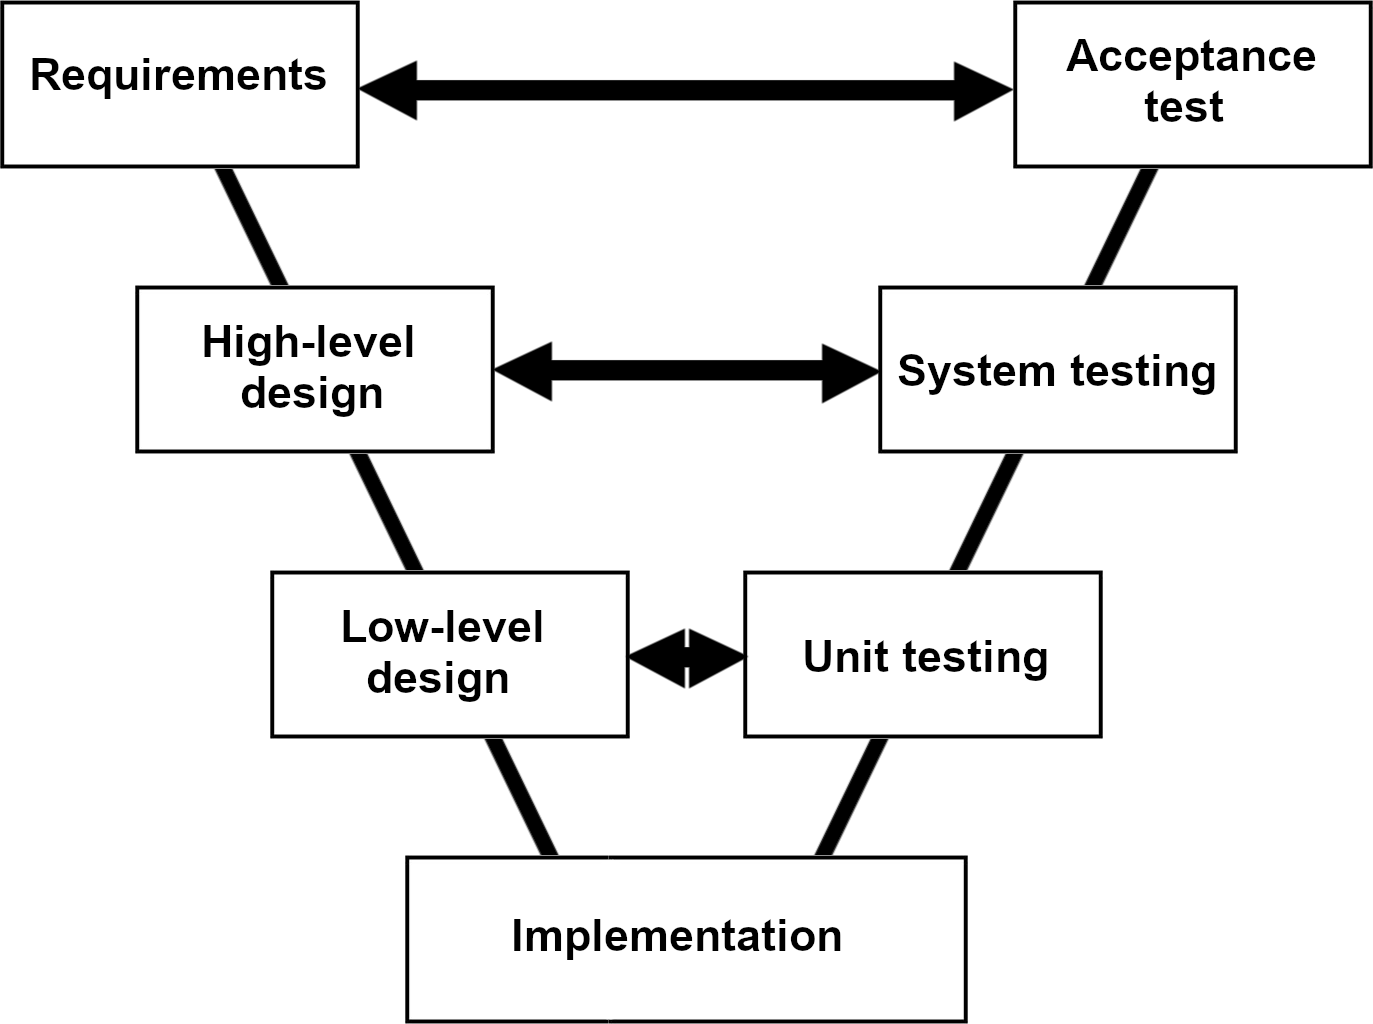
\includegraphics[width=0.7\linewidth]{img/vmodel}
	\caption{V-Model diagram}
	\label{fig:vmodel}
\end{figure}


\section{Report outline}
%TODO: add after everything else is done
%After the introduction, the report can be split into three parts, each corresponding to one of the phases in the waterfall model from Figure \ref{fig:phases}. 

%The functional design chapter introduces all the necessary prerequisite knowledge, which has been explored during the familiarization and research. It also describes the design process as the project moved from research to implementation. 

%After that, the technical design discusses the most important implementation and integration details. It also discusses practical details that might be useful for future work.

%The last three chapters, testing results, conclusion and recommendations, show the outcomes of the tests and present the explanation of those results. They also contain advice for future work, motivated by the test data interpretation and the conclusions drawn from them.

%The appendices are not integral to the report, but might prove useful to people looking to expand on the project.